
\lhead[\chaptername~\thechapter]{\rightmark}

\rhead[\leftmark]{}

\lfoot[\thepage]{}

\cfoot{}

\rfoot[]{\thepage}

\chapter{Hierarchical CNN}
\label{HierCNN}

\begin{figure}
    \centering
    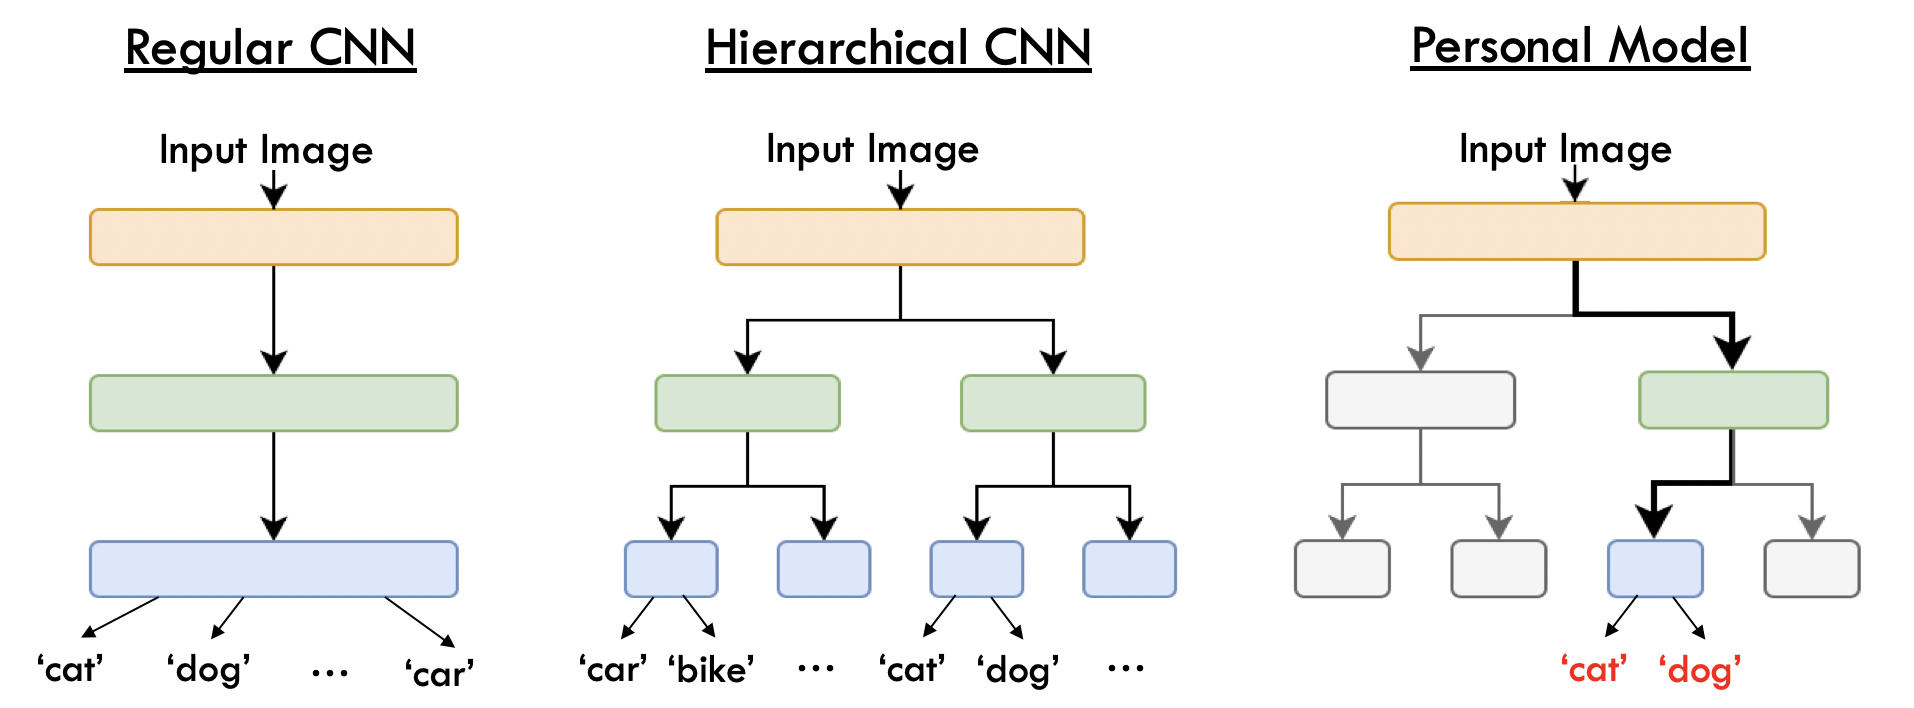
\includegraphics[width=\textwidth]{thesis/images/hierarchical-cnn-fig.png}
    \caption{Regular CNN model on the left is converted to a hierarchical CNN. Users can use only some branches depending on their needs.}
    \label{fig:hiermethodoverview}
\end{figure}

Given a regular CNN model that can recognize many class categories, our method designs a hierarchical CNN which can be used partially according to each user's requirements. 
As it can be seen in the figure \ref{fig:hiermethodoverview}, users are able to use only a single branch of the hierarchical model if they only require a few categories, such as cats and dogs in this case. 
In this way, our method is trying to achieve smaller, memory efficient CNN models that are adapted to each user's personal usages.

There are two steps in our method: creating a hierarchical representation of class categories and building CNN model according to the hierarchy.
In the following subsections, firstly our method will be explained in detail.
Secondly, we explain the process of building the hierarchy and CNN model. 
Then, the details of generating realistic training and test users are shared.
Lastly, we define the baselines to compare with our method.

\section{Method}

In a traditional classification task, a classification model $M$ takes an image $\mathbf{I}$ and generates an output $y\in\mathcal{C}$ with $\mathcal{C} = \{1,2,\dots,C\}$ where $C$ is number of different classes in a dataset. Our goal is to reduce the size of the model $M$. In the following paragraphs, 

User requirements are represented for the each user as $\mathcal{U} \subseteq \mathcal{C}$. 
Given a user requirement $\mathcal{U}$, we want to obtain $M_u$ where $M_u(\mathbf{I}) = c$ and $c\in\mathcal{U}$. 
More importantly, we expect $M_u$ to be smaller than $M$ size, therefore more memory efficient. 
However, traditional CNN models are not separable to smaller models.

Our method builds a hierarchical CNN so that each user can use only a few required branches according to their required labels. 
According to the figure \ref{fig:hiermethodoverview}, the left model $M$ is converted to the hierarchical model. 
Given the user requirements $\mathcal{U}$ as the labels of "cat" and "dog", only the highlighted branch at the right, $M_u$, is loaded into the user's device. 
Our final goal is that the average size of each user model $M_u$ is less than $M$.


\subsection{Constructing the hierarchy}
\label{ssec:hierarchy}

According to our assumption, there is a high correlation between some pairs of classes in the sense that 
if users encounter a class, they are also likely to encounter another class if they are correlated. 
For example, in object recognition task, if users detect a computer, they are likely to detect a desk as well. 
By using this correlation, our objective is to place highly correlated classes closer in the hierarchy, 
so that users are most likely to find all the classes they need in nearby branches. 
As a result, users would use less branches and therefore less memory.

Hierarchy is determined according to the correlation between pairs of classes. 
Correlation between classes can be observed from the usage of a classification model for many users.
Given user data with encountered images $\mathcal{D}_\mathrm{image} = \{\mathbf{I}_1,\mathbf{I}_2,\dots\}$ and their corresponding classification labels $\mathcal{D}_\mathrm{label} = \{c_1,c_2,\dots\}$, we can count the occurrences of each class label $c$.
Let us also define the co-occurrence matrix for a single user data as $\mathbf{O}_u = (o_{ij})\in\{0,1\}^{CxC}$ where
\begin{equation}
o_{ij} =
\begin{cases}
1~~\mathrm{if}~~c_i\in\mathcal{D}_\mathrm{label}~~~~and~~~~c_j\in\mathcal{D}_\mathrm{label}\\
0~~\mathrm{otherwise}
\end{cases}
\end{equation}
By adding the co-occurrence matrices for each user, we obtain overall number of co-occurrences for each pair of class labels, $\mathbf{O} = \sum_u \mathbf{O}_u$.
$\mathbf{O}$ matrix can be interpreted as similarity between the class labels. 
The higher the number, the more times the corresponding pair is observed together by the same user.
Therefore, $1/o_{ij}$ can be used to define the distances between each pair of class labels.
By using the distances, top-down hierarchical clustering approach would be to divide the labels into 2 using a clustering algorithm such as k-means. 
Then, the whole hierarchy can be obtained by applying clustering algorithm recursively.
On the other hand, bottom-up approach is considering every label as a cluster at first. 
Joining the clusters with the smallest distance and continue joining every cluster until they are all connected.
In our work, we used the bottom-up hierarchical clustering approach.
10-class example can be seen in the figure \ref{fig:hierarchy}.

\begin{figure}
    \centering
    \begin{minipage}[b]{.4\textwidth}
        \centering
        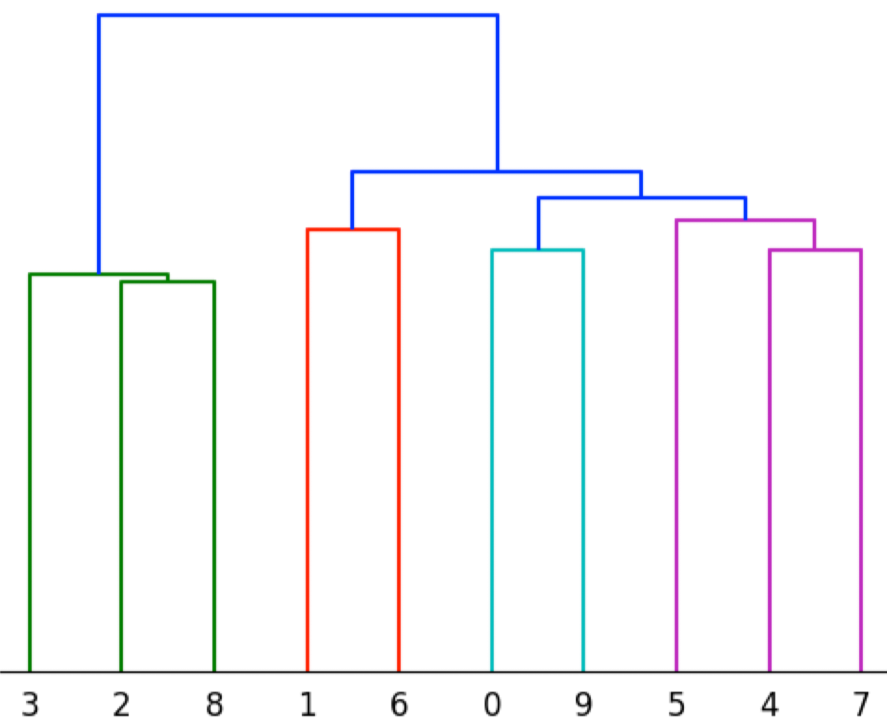
\includegraphics[width=.9\linewidth]{images/hierfig.png}
        %\caption{Hierarchical clustering of each class label in a 10-class example}
    \end{minipage}%
    \begin{minipage}[b]{.4\textwidth}
        \centering
        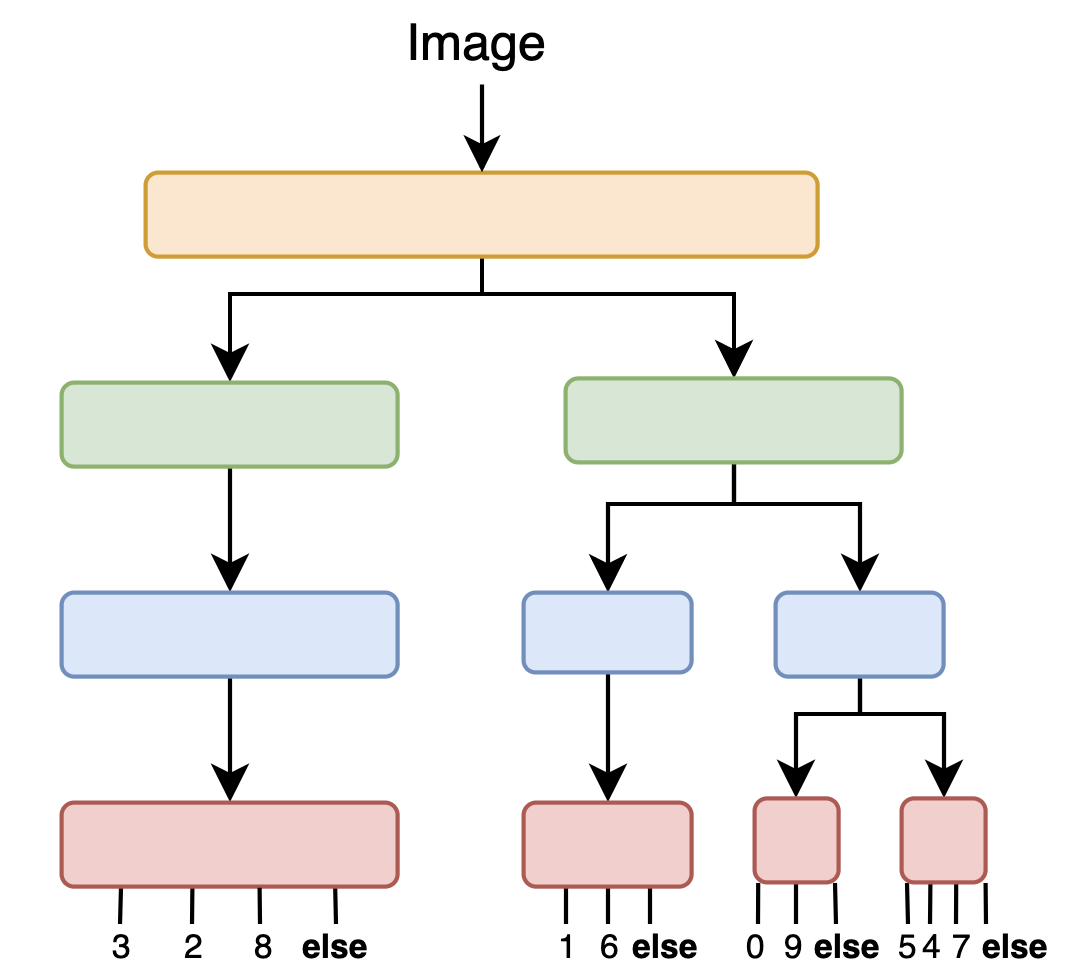
\includegraphics[width=.9\linewidth]{images/example_hier.png}
        %\caption{Hierarchical CNN obtained from the hierarchy on the left}
    \end{minipage}
    %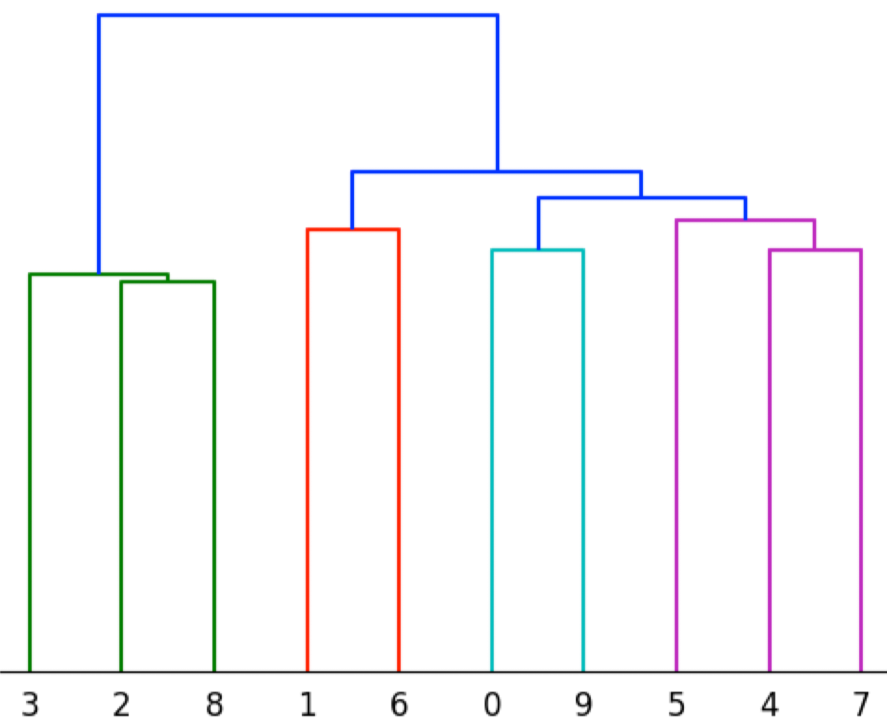
\includegraphics[width=0.40\textwidth]{images/hierfig.png}
    \caption{Hierarchical clustering of each class label in a 10-class example and the resulting network structure}
    \label{fig:hierarchy}
\end{figure}

\subsection{Hierarchy to CNN model}
\label{ssec:hiertoCNN}

Obtaining the hierarchy as described in \ref{ssec:hierarchy}, we construct our hierarchical CNN model. Depending on the hyper-parameters, such as depth of the tree, branching positions etc., there are many ways to construct the structure of hierarchical CNN with reference to the obtained hierarchy.

The structure is designed as a binary tree-shaped CNN, where the input image enters through the root layer.
Each layer takes the result of its parent layer as input and forwards its output to the next layer. 
Following the final output of the leaf layer is the classification layer for the subset of classes corresponding to that specific branch.
Note that, an extra classification label called 'else' is added to each leaves to detect classes that do not belong to a specific branch.
In the real-life scenario, if a user's model gives the output 'else', it means the encountered image has the class label that the user's model does not include.  
Therefore, additional model parts are downloaded until the image is recognized.

When constructing the tree-structured CNN, we followed some constraints as follows. 
In general, tree-structured CNN is designed by following a backbone network, such as VGG16 or MobileNet, as the base network, and branching it recursively to obtain a tree version of the network.
The structure is designed to be a binary tree, meaning a layer can only branch into two layers. 
Moreover, every path from the root to each leaf follows the same order of layers with the layer order of the backbone network.
Finally, the size of the resulting tree-structured CNN and the corresponding backbone network must be comparable. 
The reason is that if users end up using the entire tree-structured CNN, they would require only as much storage as the original backbone network.
To achieve this, after each and every branching, the number of convolutional channels in the following layers are reduced.

There are also hyper-parameters that affects the structure of the tree-based CNN. 
'Depth' hyper-parameter controls the number of times that the network can branch into two following networks. 
Moreover, 'branching positions' parameter controls where the branching happens.
For example, if the first position is '3', the network branches just after the 3rd convolutional layer in the backbone network.

In the light of all the above-mentioned constraints and hyper-parameters, the hierarchical CNN is constructed as in the figure \ref{fig:hierarchy}. 
In this simple example, the backbone network consists of four subsequent convolutional layer modules. 
'Depth' is set as 3 and 'branching positions are set as 1,2,3. 
Note that, reduced number of convolutional channels are represented as the size of the layers in the figure.
As an implementation rule, we do not split the branch if the remaining class labels in the branch is 3 or less. 
That is why the left branch in the figure is not divided into further sub-branches.

\section{Experiments}

\subsection{Generating user types and case study users}
\label{ssec:genusers}

Our method requires training users to create the hierarchy of our model as described in section\ref{ssec:hierarchy} and test users to test the final model in a scenario-based approach. 
We generated user data artificially in our work, therefore a realistic generation method is followed.
In our work, user data is defined as $\mathcal{D}_\mathrm{image} = \{\mathbf{I}_1,\mathbf{I}_2,\dots\}$, where each element represents an images a user encounters in their daily life. 
$\mathcal{D}_\mathrm{label} = \{c_1,c_2,\dots\}$ are the corresponding classification labels.
We can use as $\mathcal{D}_\mathrm{label}$ for obtaining the hierarchy as encountered labels are more important for training the hierarchy.

Our main assumption is that users interact with some classes significantly more than they interact with others due to their surroundings. 
Let us define the probability of users encountering class labels as $P=(p_1, \dots, p_C)$ where $\sum_{j=1}^C p_j = 1$ and $C$ is the number of different class labels.
To obtain these probabilities, we used Dirichlet distribution where the parameters of Dirichlet distribution are $(\alpha_1, \alpha_2, \dots, \alpha_C)$. 
The larger the $\alpha$ value is, the higher the probability output for the corresponding class label.
The output of the Dirichlet distribution determines each $P$.
We will refer to $P$ as user types for the rest of the paper.
All users will be generated according to one of the user type probabilities. 
User types can be interpreted as people with different surroundings, 
for example a chef is surrounded by kitchen tools whereas a pilot encounters airplanes on a daily basis.
Therefore, some probabilities are significantly higher than the others.

When choosing Dirichlet distribution parameters, we randomly put high values (200s) for more likely to encounter classes and low values (1s) for less likely to encounter classes. An example in 5-class classification would be $Dir(1,1,200,1,200)$. 
User type generated from this distribution will have high probability values corresponding to 3rd and 5th class labels.
A user generated from this user type will encounter images with class labels 3 and 5 much more than the rest of them. 

In our experiments with CIFAR-10, we randomly put 200s to 2 or 3 indices, which means users are likely to encounter 2 or 3 classes out of 10.
After creating the user types, users are generated, randomly following one of the user type probabilities $P$.
To generate a single user, a user type is chosen uniformly randomly between all user types. 
Then, set of encountered class labels for users, $\mathcal{D}_\mathrm{label} = \{c_1,c_2,\dots\}$, are generated according to the chosen user type. 
An example of list of encountered class labels would be, ${3,3,5,3,5,5,\dots,2,\dots,3,5,3}$ if generated from the distribution $Dir(1,1,200,1,200)$. 
It can be interpreted as the user usually encounters 3rd and 5th classes and sometimes encounters other classes as well.
Finally, random images from the dataset are collected corresponding to the class categories in the list to make scenario-based test users, $\mathcal{D}_\mathrm{image} = \{\mathbf{I}_1,\mathbf{I}_1,\dots\}$.

On a final note, training users are generated to construct the hierarchy of the system, whereas test users are generated to test our model as a scenario-based approach. 
Both training and testing users are from the same user types as we assume correlation between the requirements of all users. 

\begin{figure}
    \centering
    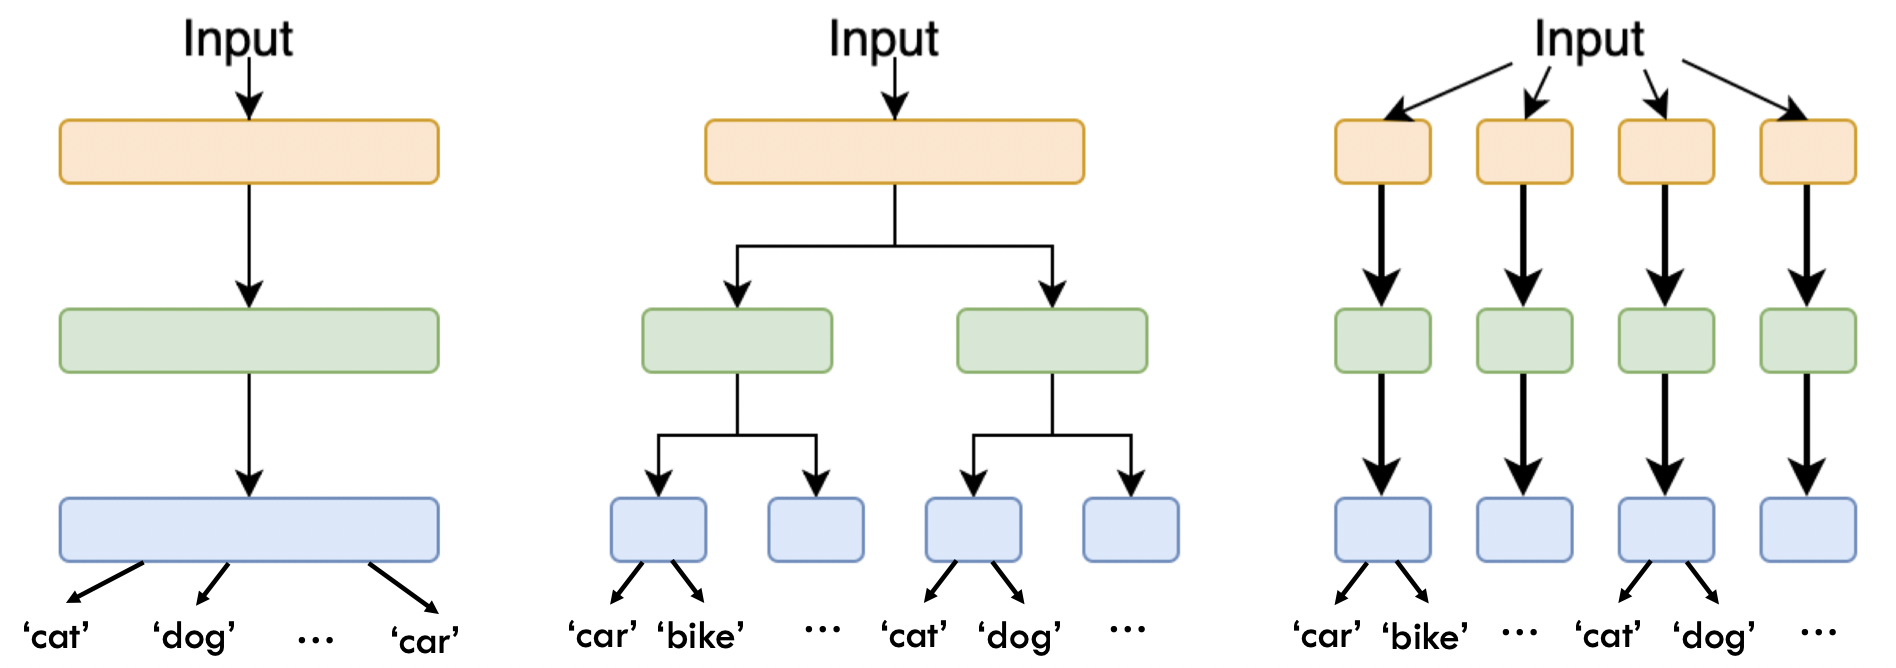
\includegraphics[width=0.9\textwidth]{thesis/images/classification_baselines-fig.png}
    \caption{Left is the regular CNN model. Middle one is the proposed hierarchical CNN. Right is the multiple smaller regular CNNs. Note that, all models are comparable in size.}
    \label{fig:baselines}
\end{figure}

\subsection{Baselines}
\label{ssec:baselines}
The whole network size of the hierarchical CNN and the baseline networks are approximately equal, because it would be fair to compare the networks with similar number of parameters. 
We constructed the hierarchical CNN simply by following a backbone network's layer order and splitting into sub-branches according to the obtained hierarchy. 

Another straightforward approach to our problem is using multiple backbone networks each reduced in size with the task of classifying a subset of classes. 
These subsets of classes corresponds to the same subsets of classes recognized in the leaf nodes of hierarchical CNN.
Same as the hierarchical CNN, we reduce the size of the each network to make the total sum of the number of parameters of all networks equal to the backbone network. 
We will refer to this method as multiple CNNs. 

In this method, none of the networks share parameters, thus decreasing the size of each network more than that of hierarchical CNNs by also reducing the number of parameters in the earlier layers. 
However, reducing the number of extracted low-level features from the input image in the early layers would result in a decrease of accuracy. 
The decrease in the accuracy is dire especially when the number of sub-networks is higher because we reduce the size of the each network more to balance with the backbone network size. 
We compare both the methods and the backbone network in terms of their accuracy and average memory consumption per user. 
All three architecture can be seen in the figure \ref{fig:baselines}.

\subsection{Dataset}

We evaluated our method on CIFAR-10~\cite{krizhevsky2009learning} dataset. 
CIFAR-10 is a relatively small dataset with 10 classes, consisting of 50000 training and 10000 test images with size 32 x 32 x 3.
The reason to choose CIFAR-10 is to try as many possibilities of constructing the hierarchy to find the best structure for the trade-off between accuracy and memory consumption.
Possible ways of constructing the Hierarchical CNN such as different depths, branching positions, etc., is tested on CIFAR-10 to find the ones with the best results with respect to both accuracy and memory cost. 
Then, in the future experiments, the best resulting models can also evaluated on bigger and more complex datasets.

\subsection{Backbone Networks}

As mentioned earlier in section \ref{ssec:baselines}, the hierarchical CNN and multiple CNNs are based on a backbone CNN, which means that they follow the convolutional layer order of another network.
In our work, VGG16~\cite{simonyan2014very} and MobileNet~\cite{howard2017mobilenets} are used as backbone networks.
Every branch starting from the root until the leaves follow the layer order of the backbone network. 
When the hierarchical CNN is split into two branches, although each branch still follows the layer order of the backbone network, the number of convolutional filters are reduced by a factor.
The reason is to maintain the overall size of the hierarchical CNN, therefore the storage consumption of the backbone network and the whole hierarchical CNN is the same which makes the comparison more fair.
Please note that, for CIFAR-10 experiments, we reduced the fully connected layer of VGG16 to prevent over-fitting, as VGG16 is designed to be used on larger domain classification problems.

\subsection{Implementation Details}

\subsubsection*{Training Phase}
Training users are generated as explained in \ref{ssec:genusers}. 
By examining the training users, the similarity between the classes can be calculated and the hierarchical clustering of class labels can be obtained, as in \ref{ssec:hierarchy}. 
Then, we construct the hierarchical CNN from the hierarchy.

When training the hierarchical CNN, every branch that leads up to a leaf node is trained with all the training images. 
Let's assume a simple example with two branches, meaning the backbone network is divided into two branches only once.
In this case, each image in the training dataset passes through the initial layers, then continues to pass the first branch and also the second branch subsequently.
Every leaf node consists of a subset of class labels and an extra label called 'else'. 
If a leaf node does not contain the class label of the training image, the branch is trained as though the label of the image is that special label 'else'. 
In our example, first the loss is calculated for the first branch and the initial layers and then the loss for the second branch and the initial layers is calculated. 
Note that, for the initial layers, loss from the first branch result and the second branch result is added to get the final loss. 
Loss calculation for more than 2 branches can be generalized in the same way.

To sum up, for each batch of training data, all branches starting from the root node and ending at a leaf node were trained together. Because some parameters between branches are shared, the shared parameters are updated according to the result of multiple leaf nodes.

\subsubsection*{Testing Phase}
In our experiments, two types of tests are conducted. 
First one is straightforward as we test the whole network of hierarchical CNN or multiple CNNs with the test set of CIFAR-10. 
The second type is the scenario-based testing, which imitates test users by using subsets of the test data.

As we emphasized throughout the paper, we assume that users encounter only a subset of all classes due to the limitation of their surroundings.
Therefore, we generated test users that are biased to encounter a subset of classes. 
The process of generating users and user types is explained in detail in section \ref{ssec:genusers}. 

For experiments on CIFAR-10, 10 user types are randomly generated and each user type is biased towards 2 or 3 random classes out of 10.
Then we generated test users that randomly belong to one of the user types. 
Each test user encounters a series of images that are biased to belong to some subset of all classes. 
Experiments are done with 100 generated test users for testing on CIFAR-10 where each test user encounters 1000 random images that are biased according to their user types.

In our scenario-based approach, users initially download the whole hierarchical model and use the whole model for the first $k$ classification task. 
This is the initial warm-up stage to learn the user's requirements.
Then, they only keep the part of the model including the formerly classified class labels and delete the rest of the model according to learned user requirements.
We will refer to the remaining part of the model as the personalized model.
In the future, if users encounter a class that is not part of the personalized model, the model detects that the newly encountered class belongs to another branch with the help of the 'else' classification label on every leaf in our tree-structured CNN (Figure \ref{fig:hierarchy}). 
As a result, they download additional parts of the model until the newly encountered class is recognized. 

The storage consumption per user is calculated as follows. 
Let us assume that a test user encounters 1000 images and personalized model was sufficient to recognize the class of the images $p$ times. 
The whole model is initially used $k$ times to learn the user requirements. 
$k$ is set to be 10 for our experiments.
The size of the whole model, personalized model and average size of the extra used model parts are $S_w$, $S_p$ and $S_{ex}$ respectively.
Then the calculation is done as the following.
\begin{equation}
    S_\mathrm{total} = [k(S_\mathrm{w}) + p(S_\mathrm{p}) + (1000-k-p)(S_\mathrm{p}+S_\mathrm{ex})] / 1000
\end{equation}
Finally, we take an average of $S_{total}$ over all the test users to obtain our final result for the storage consumption in our scenario.


\begin{table}
\begin{center}
\begin{tabular}{c||c|c|c||c|c|c}
\begin{tabular}[c]{@{}c@{}}Type of\\ Network\end{tabular} &
\begin{tabular}[c]{@{}c@{}}Number of \\ Parallel \\ Models\end{tabular} & 
Depth & 
\begin{tabular}[c]{@{}c@{}}Branching\\ Positions\end{tabular} & 
\begin{tabular}[c]{@{}c@{}}Test\\ Accuracy\end{tabular} & 
\begin{tabular}[c]{@{}c@{}}Scenario\\ Accuracy\end{tabular} & 
\begin{tabular}[c]{@{}c@{}}Number of\\ Params\\ (millions)\end{tabular}  \\
\hline\hline
VGG16& - & - & - & 89.33 & 88.38 & 15.25  \\ 
\hline
\hline
\multirow{3}{*}{\begin{tabular}[c]{@{}c@{}}Multiple\\ Smaller\\ CNNs\end{tabular}} 
& 2 & - & - & 88.54 & 88.57 & 9.9 \\ 
\cline{2-7} 
& 3 & - & - & 90.68 & 90.74 & 9.97 \\ 
\cline{2-7} 
& 5 & - & - & 89.89 & 89.78 & \textbf{7.89} \\ 
\hline
\hline
\multirow{10}{*}{\begin{tabular}[c]{@{}c@{}}Hierarchical\\ CNNs\end{tabular}} 
& - & 1 & 3 & 89.59 & 90.01 & 10.17 \\ 
\cline{2-7} 
& - & 1 & 6 & 91.08 & 90.89 & 10.33 \\ 
\cline{2-7} 
& - & 1 & 9 & 90.91 & 90.25 & 11.1 \\ 
\cline{2-7} 
& - & 2 & 3,6 & 90.69 & 90.64 & 9.52 \\ 
\cline{2-7} 
& - & 2 & 6,9 & 90.88 & 91 & 9.82 \\ 
\cline{2-7} 
& - & 2 & 3,9 & 90.58 & 90.64 & 9.72 \\ 
\cline{2-7} 
& - & 2 & 6,12 & 91 & 90.92 & 10.28 \\ 
\cline{2-7} 
& - & 2 & 9,12 & 90.79 & 90.41 & 11 \\ 
\cline{2-7} 
& - & 3 & 3,6,9 & \textbf{91.7} & \textbf{91.71} & \textbf{8.27} \\ 
\cline{2-7} 
& - & 3 & 6,9,12 & \textbf{91.75} & 91.54 & 9.11                                                                   
\end{tabular}
\end{center}
\caption[Comparison of Accuracy and Memory Cost on Image Classification task with VGG16]{\textbf{Comparison of Accuracy and Memory Cost on Image Classification task with VGG16}: Two methods are compared with the backbone network on the test accuracy, scenario accuracy and number of parameters.}
\label{ic-vgg16cifar10}
\end{table}


\subsection{Results}
As mentioned before, experiments are done on CIFAR-10. Results for the models using VGG16 as the backbone network can be seen in the Table \ref{ic-vgg16cifar10} where as results for MobileNet based models is in the Table \ref{ic-mobilenetcifar10}. 

The first three columns are the hyper-parameters. 
In this specific experiment, hierarchical CNN with depths 1, 2, 3 has 2, 3 and 5 leaf nodes or branches respectively due to the obtained hierarchy.
Also, they correspond to multiple CNNs with number of models 2, 3 and 5. 
Each corresponding model pairs have the same class labels on their leaf nodes.
Incidentally, note that depth is limited to 3 in CIFAR-10 experiments due to the number of classes.

Branching positions are generally chosen to be the convolutional layer positions that the number of kernels increase with respect to the previous layer in the backbone network. 
The reason is intuitive because otherwise the number of kernels would be less than the previous layer's as we reduce the number of kernels when branching. 
Having said that, it is also possible to choose all positions.

In both Table \ref{ic-vgg16cifar10} and \ref{ic-mobilenetcifar10}, best model overall is hierarchical CNN architecture with depth 3. 
Even though the number of parameters for multiple CNN with 5 models is the least, the accuracy drop is an issue because the number of parameters for first layers are less than that of hierarchical CNN.


\begin{table}
\begin{center}
\begin{tabular}{c||c|c|c||c|c|c}
\begin{tabular}[c]{@{}c@{}}Type of\\ Network\end{tabular} &
\begin{tabular}[c]{@{}c@{}}Number of \\ Parallel \\ Models\end{tabular} & 
Depth & 
\begin{tabular}[c]{@{}c@{}}Branching\\ Positions\end{tabular} & 
\begin{tabular}[c]{@{}c@{}}Test\\ Accuracy\end{tabular} & 
\begin{tabular}[c]{@{}c@{}}Scenario\\ Accuracy\end{tabular} & 
\begin{tabular}[c]{@{}c@{}}Number of\\ Params\\ (millions)\end{tabular}  \\
\hline\hline
MobileNet& - & - & - & 89.7 & 89.02 & 3.22  \\ 
\hline
\hline
\multirow{3}{*}{\begin{tabular}[c]{@{}c@{}}Multiple\\ Smaller\\ CNNs\end{tabular}} 
& 2 & - & - & 88.86 & 88.79 & 2.12 \\ 
\cline{2-7} 
& 3 & - & - & 88.37 & 88.43 & 2.16 \\ 
\cline{2-7} 
& 5 & - & - & 88.06 & 87.89 & \textbf{1.75}\\ 
\hline
\hline
\multirow{10}{*}{\begin{tabular}[c]{@{}c@{}}Hierarchical\\ CNNs\end{tabular}} 
& - & 1 & 3 & 89.64 & 89.46 & 2.13 \\ 
\cline{2-7} 
& - & 1 & 5 & 90.21 & 90.09 & 2.19 \\ 
\cline{2-7} 
& - & 1 & 8 & 90.09 & 89.71 & 2.45 \\ 
\cline{2-7} 
& - & 2 & 3,6 & 90.15 & 90.04 & 1.99 \\ 
\cline{2-7} 
& - & 2 & 5,8 & 90.16 & 89.84 & 2.08 \\ 
\cline{2-7} 
& - & 2 & 3,8 & 89.87 & \textbf{90.14} & 2.03 \\ 
\cline{2-7} 
& - & 2 & 5,11 & \textbf{90.6} & 90.11 & 2.18 \\ 
\cline{2-7} 
& - & 2 & 8,11 & 89.98 & 89.19 & 2.44 \\ 
\cline{2-7} 
& - & 3 & 3,6,9 & \textbf{90.27} & \textbf{90.12} & \textbf{1.82} \\ 
\cline{2-7} 
& - & 3 & 5,8,11 & 89.89 & 89.88 & 1.98                                                                   
\end{tabular}
\end{center}
\caption[Comparison of Accuracy and Memory Cost on Image Classification task with MobileNet]{\textbf{Comparison of Accuracy and Memory Cost on Image Classification task with MobileNet}: Two methods are compared with the backbone network on the test accuracy, scenario accuracy and number of parameters.}
\label{ic-mobilenetcifar10}
\end{table}

